\section{Einleitung}
% TODO Diagramm für Stellenvakanz?
Der Einsatz von Robotern prägt zunehmend den Arbeitsmarkt und beeinflusst die Art und Weise wie Unternehmen ihre Prozesse gestalten. Diese Entwicklung beschränkt sich nicht nur auf klassische Einsatzgebiete wie die Industrie, in der beispielsweise Montageroboter eingesetzt werden, und den Verbrauchermarkt, in dem Staubsaugerroboter mittlerweile weit verbreitet sind, sondern zunehmend auch auf die Dienstleistungsbranche. Ermöglicht wird diese Entwicklung durch den technischen Fortschritt in den Bereichen Robotik, \ac{KI}, Big Data, Kameras, Sensoren und Spracherkennung \cite[S.~424]{Paluch2020}. Der Absatz von Servicerobotern für professionelle Anwendungen verzeichnete laut der \ac{IFR} im Jahr 2022 einen Anstieg um 48\% \cite{IFR2023}, während der Absatz von Industrierobotern schwächer zunahm \cite[S.~9]{WorldRobotics2023} und bei Servicerobotern im Verbrauchermarkt sogar rückläufig war \cite[S.~37]{WorldRobotics2023}. Dieses Wachstum wird laut der \ac{IFR} durch eine gesteigerte Nachfrage getrieben, die unter anderem auf einen Mangel an Arbeitskräften zurückzuführen ist \cite[S.~33-34]{WorldRobotics2023}. Laut der \ac{BA} ist die Menge unbesetzter Arbeitsplätze in Deutschland in den letzten 10 Jahren um 40\% gestiegen und – trotz des Rückgangs um 18\% in den letzten zwei Jahren – weiter auf einem hohen Stand \cite{BA2024}. Insbesondere in der Gastronomie gibt es einen erheblichen Personalmangel, der zum Teil auf die Corona-Pandemie zurückzuführen ist, da in dieser Zeit viele Angestellte in andere Berufsfelder gewechselt sind. Laut dem Institut der deutschen Wirtschaft, welches sich auf Daten der \ac{BA} bezieht, sind während des Pandemiejahrs 2020 circa 216.000 Arbeiter aus dem Gastgewerbe in ein anderes Berufsfeld gewechselt \cite[S.~1]{Jansen2022}. Serviceroboter bieten durch eine effiziente Unterstützung des Personals die Möglichkeit den Personalmangel zu mitigieren. So ersetzen Serviceroboter das Personal meistens nicht vollständig, sondern unterstützen es, sodass es mehr Zeit für andere Aufgaben wie die Kundenbetreuung hat \cite[S.~271-272]{Sprenger2015}. In der Gastronomie können Lieferroboter beispielsweise bestimmte Kellner Aufgaben übernehmen und so das Personal entlasten.

\subsection{Hintergrund und Motivation}\label{sec:BackgroundAndMotivation}
In diesem Kontext hat sich die Firma Tobit Laboratories AG entschieden die Potenziale von Lieferrobotern für eigene Gastronomiebetriebe zu erkunden. So hat das Unternehmen mehrere Lieferroboter von Pudu Robotics erworben, um diese Technologie zu testen. Zur Steuerung der Roboter aber auch zur Erweiterung der Funktionen wurde das \ac{BCB} entwickelt, das im Abschnitt \ref{sec:BotControlBackend} näher erläutert wird. Zur Prüfung der Eignung sollen die Roboter zunächst im Firmengebäude für kleinere Botengänge eingesetzt werden. Hierfür müssen die Roboter zum einen auf verschiedene Aspekte, wie die Navigationsfähigkeit und Zuverlässigkeit geprüft werden. Zum anderen muss aber auch eine Anwendung entstehen, mit der die Roboter vor allem intuitiv gesteuert, aber auch verwaltet werden können. Abhängig der Ergebnisse könnten die Roboter dann möglicherweise in verschiedenen Gastronomiebetrieben eingesetzt werden.

\subsection{Zielsetzung und Forschungsfrage}\label{sec:ResearchQuestion}
Diese Arbeit setzt an diesem Punkt an und zielt darauf ab, eine Anwendung zu konzipieren und prototypisch zu implementieren, die die Steuerung und Verwaltung von Lieferrobotern ermöglicht und zudem eine Übersicht über deren Positionen bietet. Bei der Anwendung soll es sich um eine Webanwendung handeln, da Webanwendungen im Gegensatz zu nativen Anwendungen eine plattformunabhängige Nutzung und sofortigen Verfügbarkeit ohne Installation bieten \cite{AWSWebApp}. Für eine möglichst übersichtliche Darstellung der Roboterpositionen sollen 3D-Modelle der Räume genutzt werden. Um eine reibungslose Integration der Roboter in Gastronomiebetriebe zu ermöglichen, sollte die Erstellung der 3D-Modelle mit minimalem Aufwand verbunden und möglichst unkompliziert sein. Hierbei gilt es zu beachten, dass die Erzeugung der 3D-Modelle nicht in dem zu entwickelnden Prototyp integriert werden muss. Trotz des erhöhten Rechenaufwands, der mit der Darstellung von 3D-Modelle verbunden ist, soll die Anwendung außerdem performant sein.

Aus dieser Zielsetzung ergibt sich die folgende Forschungsfrage: Wie kann eine effiziente und benutzerfreundliche Steuerung und Verwaltung von Servicerobotern implementiert werden?

\subsection{Methodik}
Um die Forschungsfrage zu beantworten wird nach dem \ac{DSR} Ansatz nach Hevner geforscht \cite{Hevner2004}. Bei diesem handelt es sich um einen iterativen Forschungsansatz, mit dem Lösungen für praktische Probleme durch die Entwicklung von Artefakten gefunden werden. Im Rahmen dieser Arbeit ist der zu entwickelnde Prototyp das Artefakt.

\subsubsection{Design Science Research nach Hevner}
Bei diesem Abschnitt handelt es sich um eine Zusammenfassung des \ac{DSR} Ansatzes nach Hevner \cite[S.~79-81]{Hevner2004}. Hevners Ansatz setzt sich aus drei Schleifen zusammen, wobei die Relevanz- und Strenge-Schleifen nur unterstützende Funktionen für die eigentliche Entwicklung – die Design-Schleife – bieten:

\begin{itemize}
    \item Die Relevanz-Schleife ergibt sich daraus, dass sich die Anforderungen an das Artefakt aus der Umgebung, für die es entwickelt wir, ergeben und das entwickelte Artefakt daraufhin in der Umgebung getestet wird. Die Umgebung ergibt sich hierbei aus den Menschen und Organisationen, die das Artefakt nutzen sollen und den Technologien, die im Artefakt eingesetzt werden sollen.
    \item Die Strenge-Schleife ergibt sich daraus, dass während der Entwicklung und Auswertung des Artefakts auf die Wissensbasis zurückgegriffen wird und diese durch die Entwicklung und Evaluierung erweitert wird. Diese Wissensbasis besteht hierbei sowohl aus dem technischen Wissen, dass während der Entwicklung relevant ist, als auch aus dem Wissen über Methodologien, die während der Auswertung relevant sind.
    \item In der Design-Schleife wird das Artefakt iterativ entwickelt. So wechselt sich das Entwickeln und Auswerten des Artefakts regelmäßig ab, bis ein befriedigendes Ergebnis erreicht wurde.
\end{itemize}

In der Abbildung \ref{fig:DesignScienceResearch} werden die beschriebenen Prozesse grafisch dargestellt. So zeigt die Abbildung die Relevanz- und Strenge-Schleifen als Unterstützungsprozesse für die eigentliche Forschung in der Form der Design-Schleife.

\begin{figure}[H]
    \caption{Design Science Research nach Hevner}\label{fig:DesignScienceResearch}
    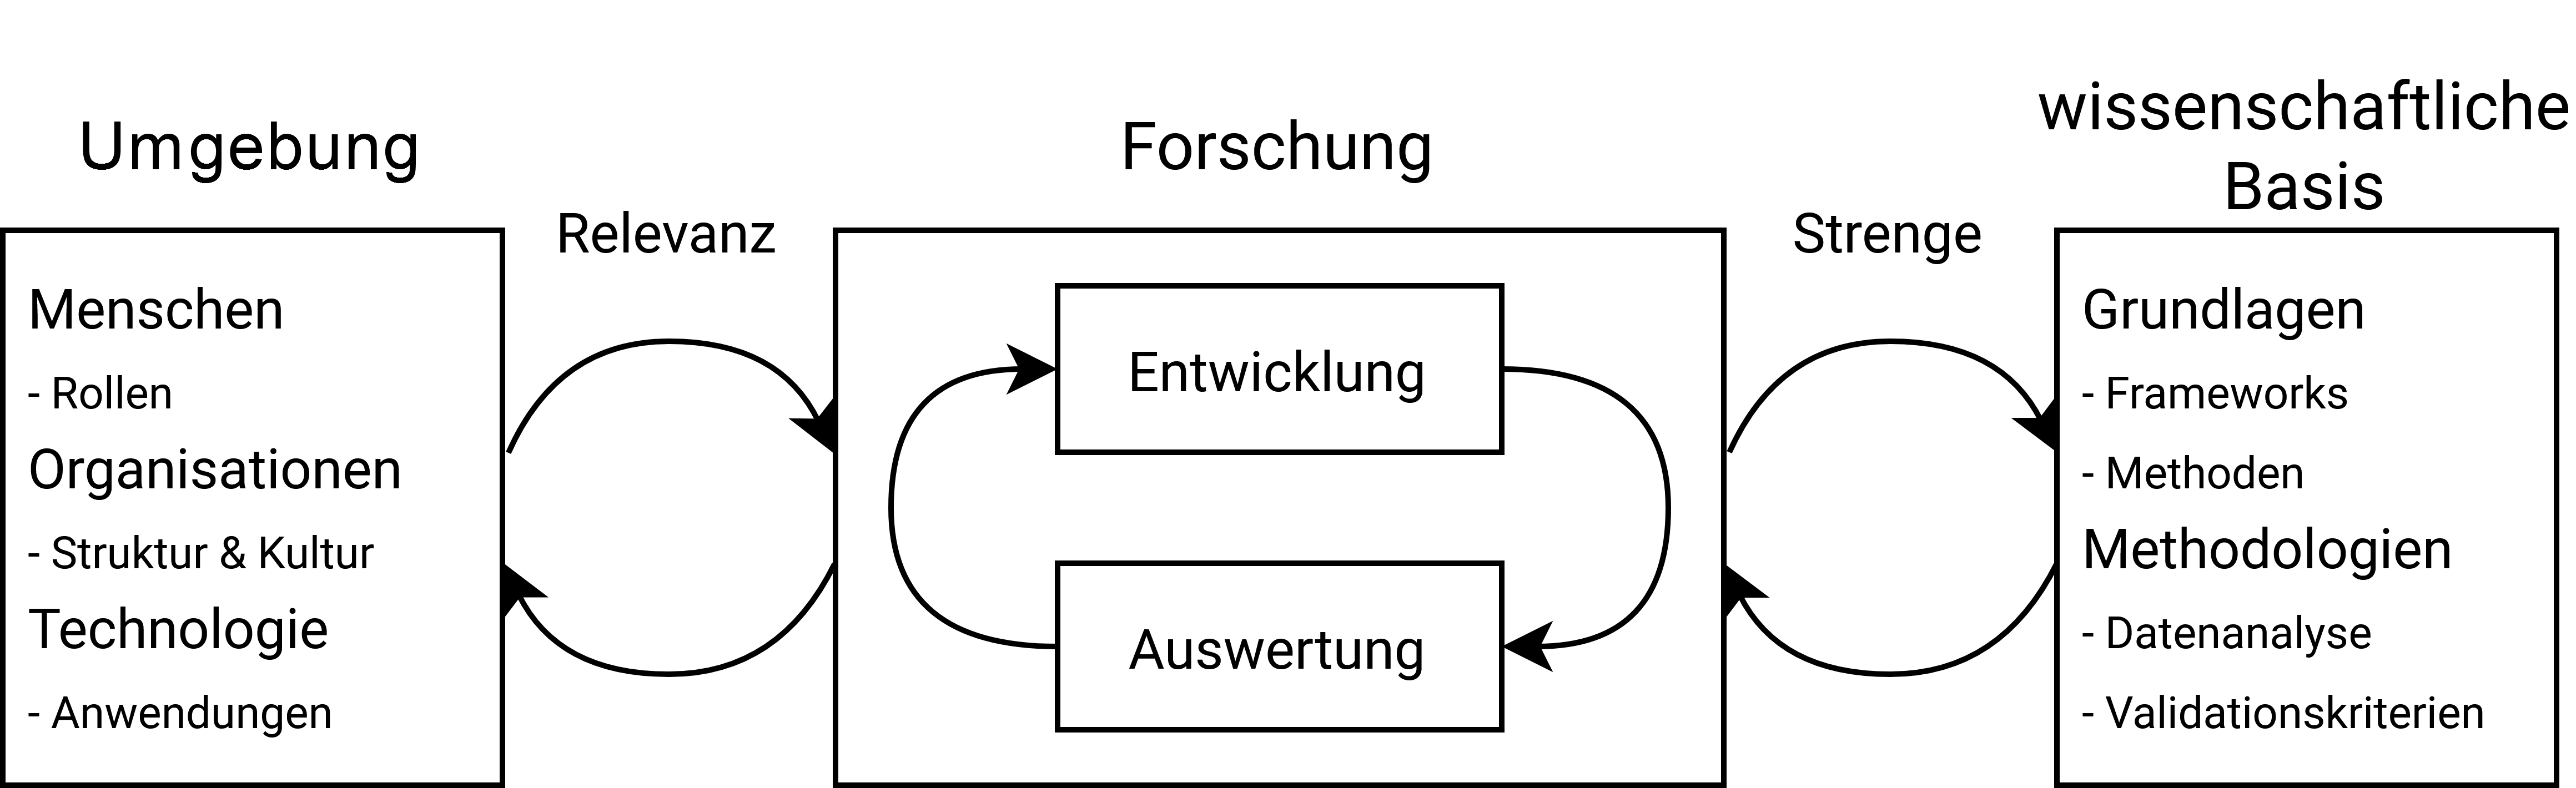
\includegraphics[width=0.9\textwidth]{Design Science Research.png}
    \\
    Quelle: In Anlehnung an Hevner et al. \cite[S.~80]{Hevner2004}
\end{figure}

\subsubsection{Design Science Research im Rahmen der Arbeit}

Die Prozesse des \ac{DSR} Ansatzes nach Hevner werden in dieser Arbeit durch verschiedene wissenschaftliche Methoden abgebildet. Im ersten Schritt wird eine systematische Literaturrecherche durchgeführt, mit der das grundlegende Verständnis über die Umgebung geschaffen und die bereits vorhandene Wissensbasis erweitert werden soll. So wird unter anderem Wissen zu Servicerobotern, zur Generierung von 3D-Modellen und zur wissenschaftlichen Auswertung von Software-Anwendungen gesammelt. Während der Entwicklung des Prototyps weitet sich diese Literaturrecherche auf die Lösung auftretender Problemen aus. Die Anforderungen, die sich aus der Umgebung ergeben werden nach der Wissensfindung durch eine Anforderungsanalyse definiert. Diese kann auf die Anforderungen aufgebaut werden, die sich bereits aus der Zielsetzung und der Formulierung der Forschungsfrage ergeben. So stehen die Anforderungen, dass der Prototyp eine Webanwendung sein und eine dreidimensionale Visualisierung bieten soll bereits fest. Auch steht bereits fest, dass der Prototyp benutzerfreundlich und effizient sein soll. Die Implementierung des Prototyps wird nach dem Verfahren des Evolutionary Prototypings durchgeführt. So wechseln sich die Entwicklung und Auswertung der Benutzerfreundlichkeit und Effizienz iterativ ab bis ein Prototyp entstanden ist, der die definierten Anforderungen ausreichend erfüllt.
% TODO Quelle Evolutionary Prototyping
